\section{Konkretes Datenmodell}
\label{sec:concrete_model}

Thema dieses Abschnittes ist die Struktur und die verwendeten Entwurfsmuster in den Datenmodellen, die die Ein- bzw. Ausgabedaten des Generators beinhalten.

\subsection{REST-Modell}
\label{sec:rest_model}

Zuerst muss die abstrakte Beschreibung der Spreadshirt-API von der XML-Form, bestehend aus einem \emph{WADL} (\cref{sec:wadl}) und einem oder mehreren Schemabeschreibungen (\cref{sec:document_description_formats}), in ein für den Generator verarbeitbares Format überführt werden.

Die durch die WADL-Datei beschriebene Baumstruktur muss in ein Datenmodell bestehend aus Klassen und Objekten transformiert werden.
Um effektiv mit der XML Darstellung arbeiten zu können wird diese zuerst mit einem Parser in ein DOM-Modell überführt (\cref{sec:xml_parser}) welches im Arbeitsspeicher gehalten wird und damit einen schnellen Zugriff für nachfolgende Operationen darauf erlaubt. In einem nächsten Schritt wird das DOM-Modell, welches noch viele XML-Dokument spezifische Informationen enthält, auf die wesentlichen API beschreibenden Merkmale reduziert. Im Gegensatz zu der in \cref{fig:wadlstructure} veranschaulichten Webanwendungsbeschreibung werden Referenzen durch deren Definition im Modell ersetzt.

\begin{figure}[tb]
    \begin{center}
        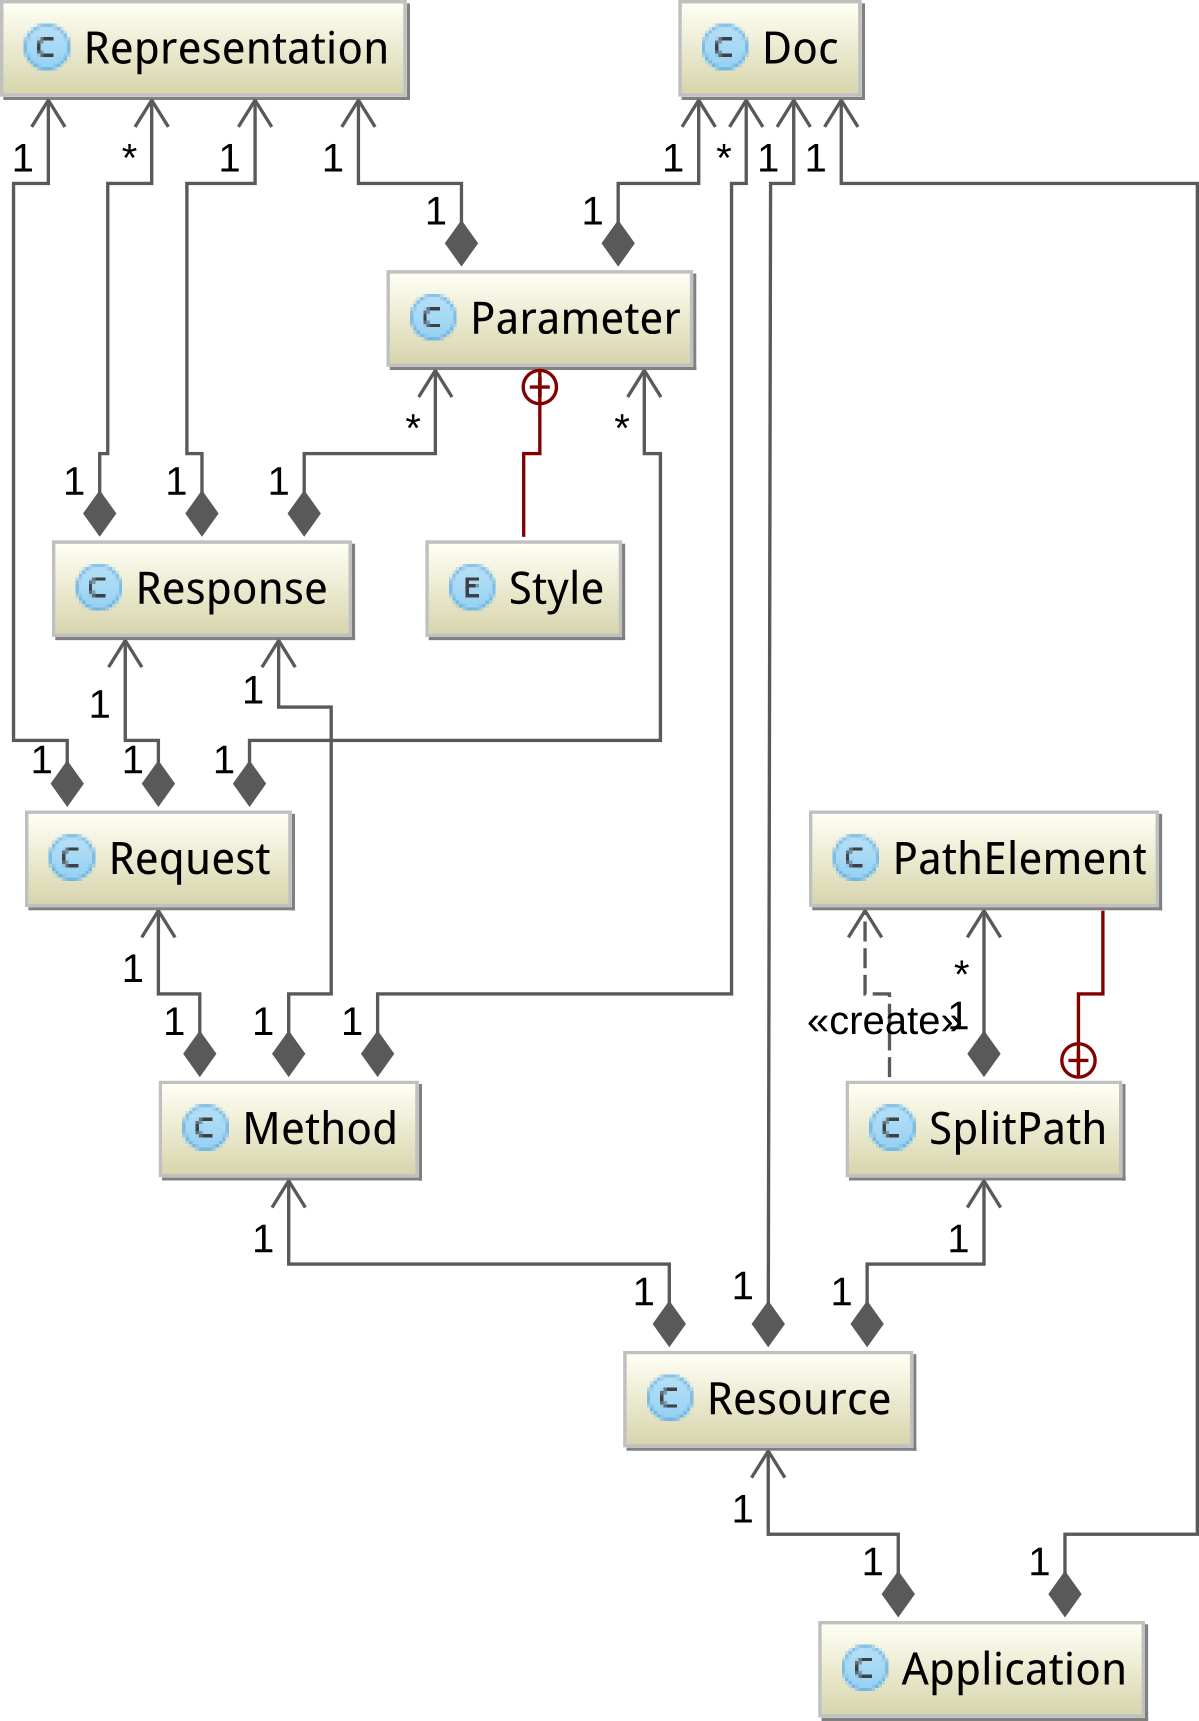
\includegraphics[width=0.5\textwidth]{resources/restmodel}
    \end{center}
    \caption{UML-Diagramm des REST-Modells}
    \label{fig:restmodel}
\end{figure}

Wurzelelement des Modells ist \textbf{Application}, über dieses Element kann auf alle \emph{Ressourcen} zugegriffen werden. Es enthält außerdem den Basisbezeichner der API bspw. \texttt{http://api.spreadshirt.net/api/v1/}. 

Eine \textbf{Ressource} enthält eine Menge von \emph{Methoden}, sowie einen Ressourcenbezeichner, diese sind relativ zum Basisbezeichner des Wurzelelements. Die Ressourcenbezeichner können \emph{Template-Parameter} enthalten, diese werden bei einer Anfrage durch einen konkreten Wert ersetzt. Beispielweise enthält der Bezeichner für die Ressource eines bestimmten Users den Template-Parameter \{userid\}, vollständiger Ressourcenbezeichner \texttt{users/\{userid\}}. Ressourcenbezeichner werden durch \textbf{SplitPath} repräsentiert. 

Jede Methode enthält ein \textbf{Request} und ein \emph{Response} Element, welche die nötigen Informationen für eine Anfrage auf bzw. den Aufbau der Antwort von, einer Ressource enthalten.

\textbf{Request} enthält eine Liste von Query-Parametern sowie ein \emph{Representation} und \emph{Response} Element.

\textbf{Parameter} enthält Angaben zum \emph{Style}, Typ, Vorgabewert und ob dessen Angabe \enquote{required}, also notwendig ist. Die Angabe des Typs ist eine Referenz auf einen Typ aus einer XML-Schemabeschreibung. Der \emph{Style} gibt an wie der Parameter übermittelt wird, als Teil der Query \texttt{\ldots{}?mediaType=xml}, \emph{Key-Value Pair} des HTTP-Header oder als \emph{Template-Parameter} des Ressourcenbezeichners. 

Das \textbf{Response} Element enthält eine Menge von \emph{Representations}, sowie eine Liste von Parametern. Die \emph{Representations} enthalten die Beschreibung der Daten die bei einer erfolgreichen Anfrage an die Ressource zurückgesendet werden, sowie die der Fehlermeldung die der Client anderenfalls erhält. Zwischen einer Fehlermeldung und einer Antwort auf eine erfolgreiche Anfrage kann anhand des Wertes des HTTP-Statuscodes unterschieden werden. Erfolgreiche Antworten liefern meist einen Statuscode 200 \textbf{OK} oder 201 \textbf{Created} zurück. Die Response Parameter geben meist Einträge im HTTP-Header an, welche für den Client nützliche Informationen enthalten. Legt der Client z.B. via POST auf der Ressource \texttt{sessions} eine neue API-Session an, enthält das Feld \texttt{Location} des HTTP-Headers der Antwort, die URL auf die Ressource der angelegten Session.

\textbf{Representation} dient zur Beschreibung der Daten welche entweder zur API gesendet oder von dieser empfangen werden, sie besteht aus einer Angabe des \emph{media-type}, des HTTP-Statuscodes und eine Referenz auf die Definition des Datentyps. Die \emph{Representation} eines Request einer PUT- oder POST-Methode charakterisiert zum Beispiel den Aufbau der Daten welche der Ressource übermittelt werden, üblicherweise im HTTP-Body. Die Charakterisierung erfolgt dabei in Form einer Referenz auf einen Typ aus einer Schemabeschreibung sowie der Angabe des \emph{media-type}. Die \emph{Representation} der PUT-Methode auf Ressource \texttt{users/\{userId\}/designs/\{designId\}} enthält den media-type \texttt{application/xml} und eine Referenz auf den Typ \texttt{sns:design}. 

Referenzen auf Typdeklaration aus einer Schemabeschreibung werden nachfolgend im Modell durch die konkrete Deklaration des Typs aus der XML-Schemabeschreibung ersetzt, siehe \cref{sec:application_model}. \textbf{Doc} Element enthalten nur einen Titel und eine Kurzbeschreibung des zugehörigen Elements. Aus dieser \emph{Dokumentation} wird durch den Generator in ein Kommentar erzeugt.

\subsection{Schema-Modell}
\label{sec:schema_model}

\subsection{Applikationsmodell}
\label{sec:application_model}

\subsection{Zielsprachenmodell}
\label{sec:abstract_target_language_model}

\subsection{PHP-Zielsprachenmodell}
\label{sec:php_target_language_model}

% Sprachschnittstelle!
\subsection{Language Factory}
\label{sec:language_factory}
